\newcommand{\problemDetail}{
Für eine sichere und korrekte Erkennung von Übermüdung ergeben sich mehrere Problemstellungen (Abb. \ref{fig:ddd_problem}). Anzeichen von Müdigkeit müssen vom System genau analysiert werden, um eine sichere Aussage über die Fahrtauglichkeit des Fahrers treffen zu können. Erkennt das System eine gefährliche Situation, muss der Fahrer in geeigneter Weise darauf hingewiesen werden.

\begin{figure}[h] 
  \begin{center}
    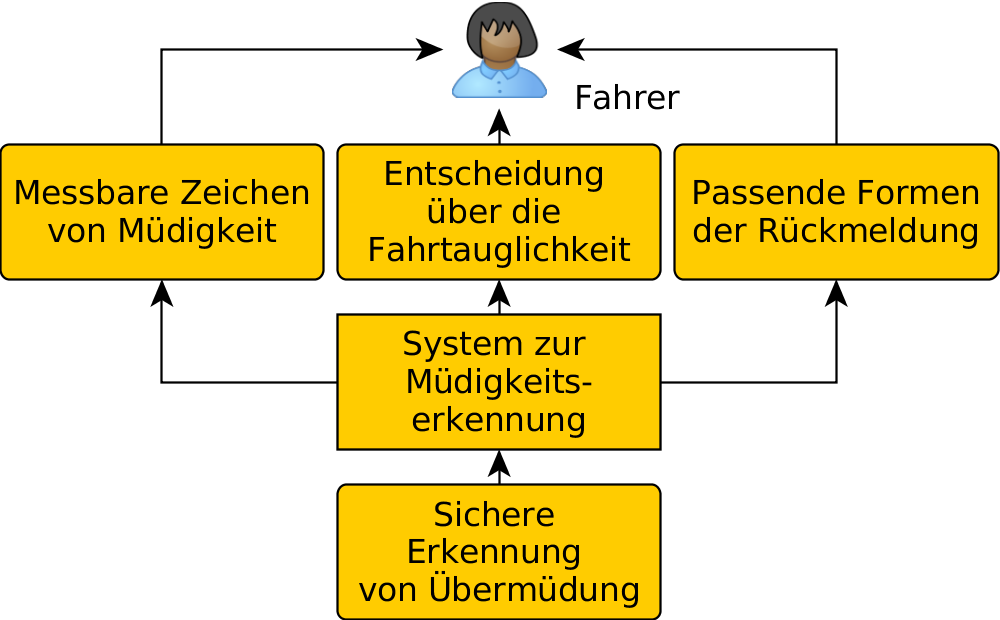
\includegraphics[width=0.75\columnwidth]{ddd_problem_detail}
    \caption[Problemstellung der Müdigkeitserkennung]{Das System zur \acl{ME} gliedert sich in mehrere Teilproblemstellungen auf.\label{fig:ddd_problem}}
  \end{center}
\end{figure}
}

\newcommand{\drivingTask}{
Abb. \ref{fig:driving_task}.

\begin{figure}[h] 
  \begin{center}
    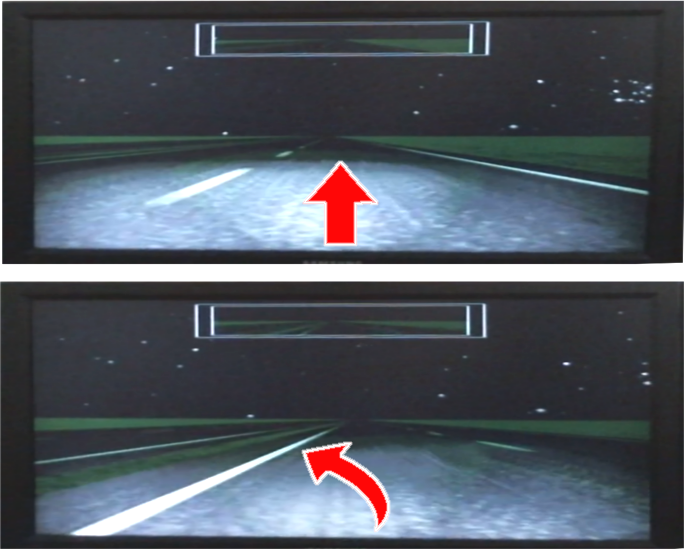
\includegraphics[width=0.6\columnwidth]{driving_task}
    \caption[Driving Task Spurwechsel]{Oben: Am Anfang fährt der Fahrer noch geradeaus auf der rechten Spur. Unten: gegen Ende kommt der Fahrer sogar von der linken Spur ab und fährt beinahe auf den Mittelstreifen \label{fig:driving_task}}
  \end{center}
\end{figure}
}

\newcommand{\rawHisto}{
 (Abb. \ref{fig:raw_histo}).

\begin{figure}[h] 
  \begin{center}
    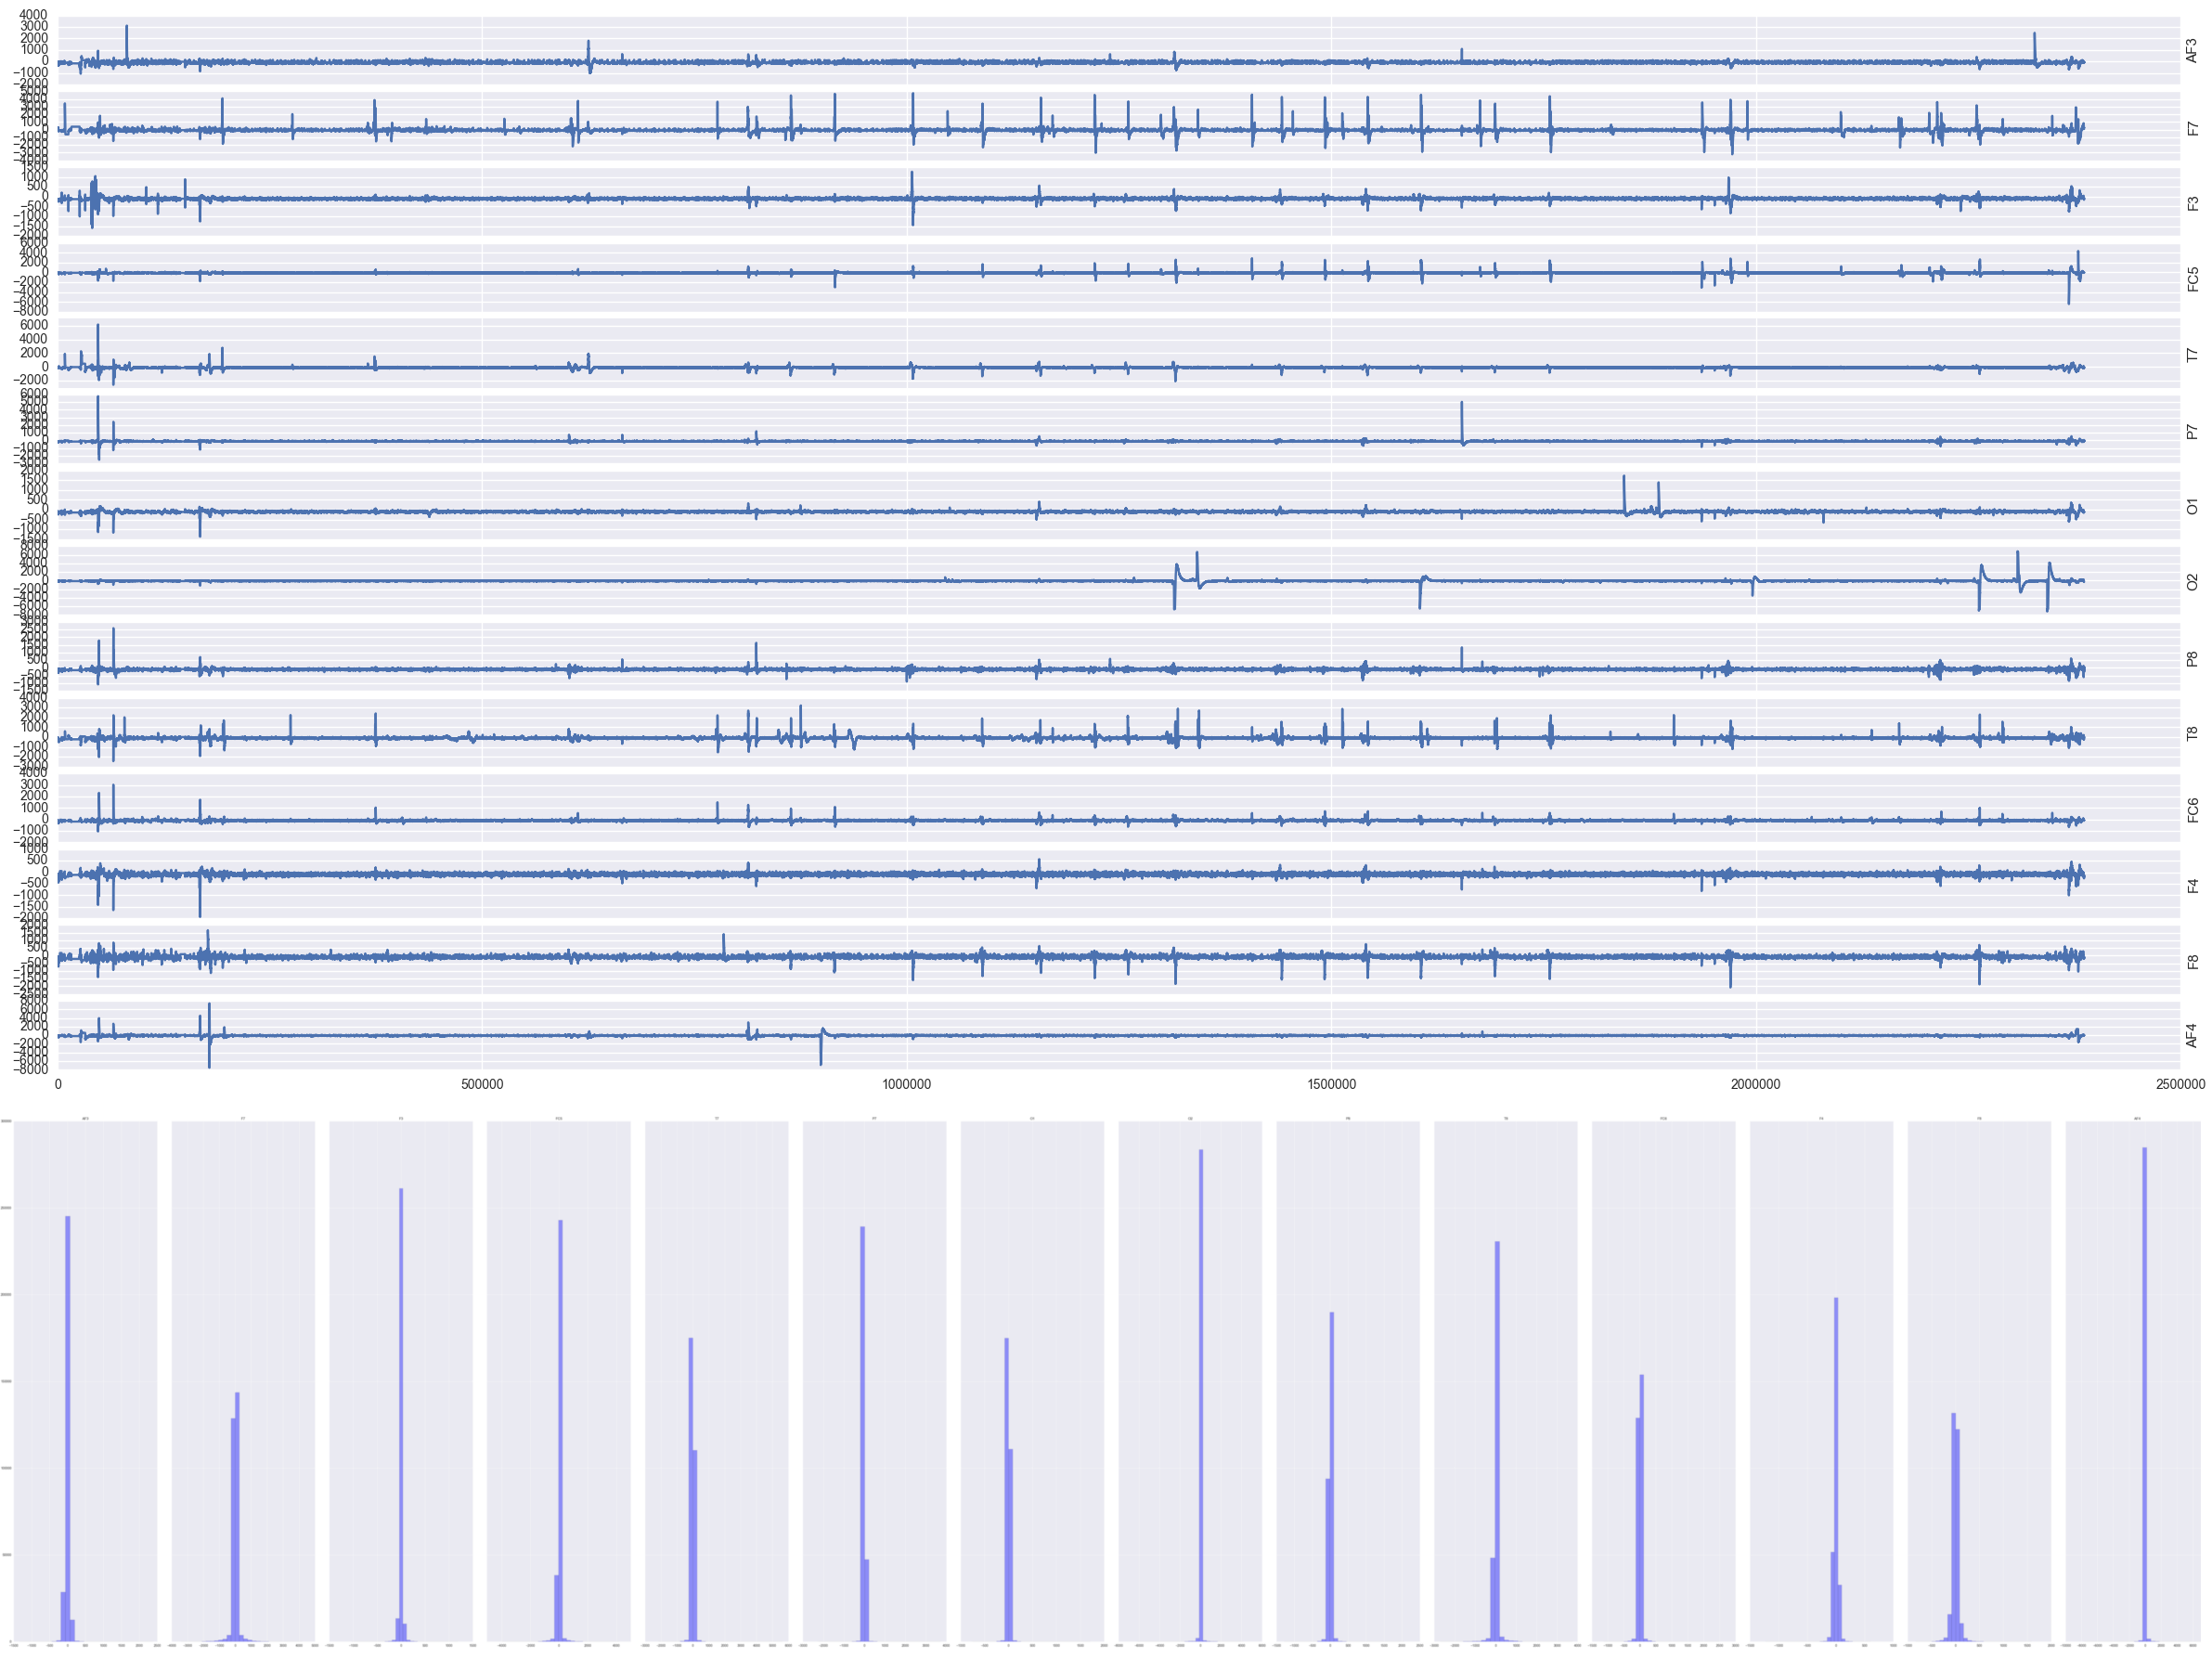
\includegraphics[width=\columnwidth]{raw_histo}
    \caption[Rohsignal und Histogramm]{Die Rohsignale pro Sensore und das dazugehörige Histogramm. Die Werte verteilen sich zwischen -8000 bis 8000, ein deutliches Maximum im Histogramm ist zwischen -100 und 100 erkennbar.  \label{fig:raw_histo}}
  \end{center}
\end{figure}
}

\newcommand{\butterworth}{
 Abbildung \ref{fig:butterworth_filter} zeigt exemplarisch Filterfunktionen verschiedener Ordnung mit den Grenzen von 500 bis 1250Hz. Alle Frequenzen darunter und darüber werden deutlich abgeschwächt bzw. gehen gegen Null.

\begin{figure}[h] 
  \begin{center}
    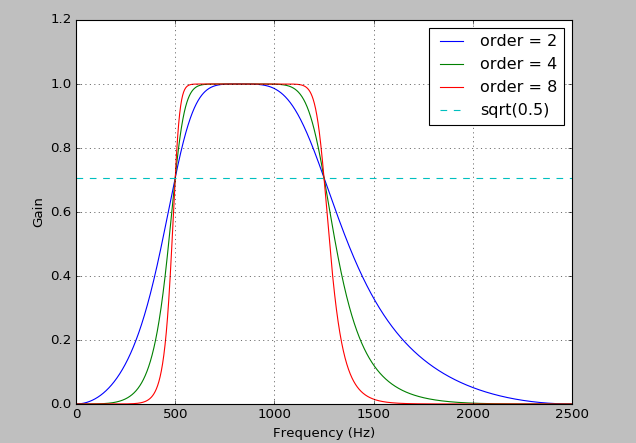
\includegraphics[width=5.5cm]{butterworth_filter}
    \caption[Butterworth-Filter]{Die Filterfunktion eines Butterworthfilters 2., 4,. und 8. Ordnung im Frequenzbereich von 500 bis 1250Hz. \label{fig:butterworth_filter}}
  \end{center}
\end{figure}
}

\newcommand{\fftExample}{
 (Abb. \ref{fig:fft_example}).

\begin{figure}[h] 
  \begin{center}
    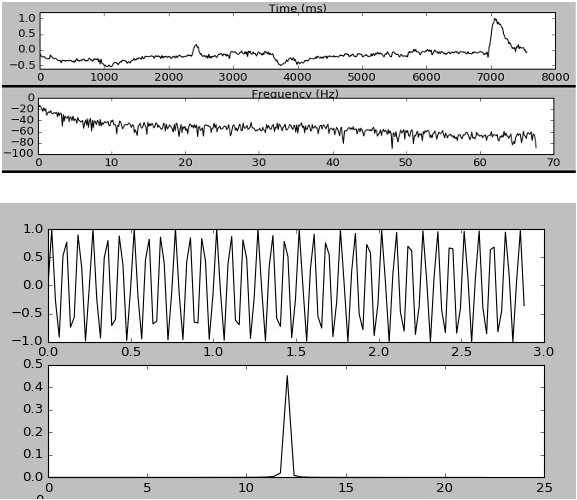
\includegraphics[width=\columnwidth]{fft_example}
    \caption[Fast Fourier Transformation]{Oben: EEG Signal darunter das Frequenzspektrum. Unten: die selbe Anordnung für ein Tonsignal und beschreibt eine Sinusschwingung mit 12KHz. Nach der FFT zeigt sich ein  Maximum bei dieser Frequenz. \label{fig:fft_example}}
  \end{center}
\end{figure}
}

\newcommand{\tofc}{
Die Ausarbeitung gliedert sich folgendermaßen: im Kapitel \ref{chap:state} werden verschiedene Forschungsergebnisse zur \acl{ME} aufgezeigt und analysiert. Daraus ergeben sich die Anforderungen an eine Anwendung zur \acl{ME}. Die Infrastruktur, die Beschaffung der Daten und die durchgeführten Versuche sind Thema von Kapitel \ref{chap:data}. Die Implementierung eines portablen Systems zur \acl{ME} mit \acl{BS} wird im Kapitel \ref{chap:implementation} vorgestellt. Kapitel \ref{chap:result} beschreibt die Ergebnisse und leitet in Kapitel \ref{chap:conclusion} zu den weiteren Schritten und dem Fazit über. Im folgenden Absatz werden Grundlagen für die kommenden Kapitel erläutert.
}

\newcommand{\comp}{
In der Praxis setzen Automobilhersteller wie Daimler\cite{Daimler} und Volkswagen, sowie Automobilzulieferer wie Bosch\cite{Bosch} auf die Analyse des Fahrverhaltens. Insbesondere das Abkommen von der Spur und ruckartiges Gegenlenken scheinen ein signifikantes Indiz für beginnende Übermüdung zu sein. Weiterhin sind externe Geräte und einige Apps für Smartphones erhältlich. Leider existieren kaum öffentlich zugängliche Arbeiten zu den verbauten Ansätzen von  \acl{ME}, da es sich um interne Entwicklungen handelt. Wissenschaftliche Artikel sind ebenfalls selten\cite{Eskandarian}.

Beim CV-Ansatz wird der Fahrer und die Straße mit Hilfe von Kameras beobachtet. Zhang et al. \cite{Zhang:2015:RSD:2753829.2629482} stellen hierzu eine Applikation mit der Microsoft Kinect vor. Es wurden sowohl die Kopfpose, als auch der Augenstatus bestimmt. Bergasa et al. \cite{Bergasa_1603553} extrahierten aus dem Bild einer Infrarot Kamera mehrere Features, wie \acl{bspw} den prozentualen Anteil von geschlossenen Augen (Percent eye closure, PERCLOS). Mit dieser Technik erreichten sie bei der Erkennung von Übermüdung eine nahezu hundertprozentige Erfolgsrate. Kamerabasierte Systeme schränken den Fahrer nicht ein, da kein direkter Kontakt zum Fahrer bestehen muss. Jedoch ist jede Kamera optischen Grenzen unterworfen (bspw. bei Nacht oder schlechtem Wetter).

Die beiden beschriebenen Bereiche werden in dieser Arbeit nur für die manuelle Markierung der aufgenommen Datensätzen genutzt. Der dritte Bereich für die Erkennung von Müdigkeit, arbeitet mit Körpersensoren bzw. deren Kombination (multimodal). Meist werden elektrische Spannung am und im Körper gemessen. Neben dem EEG, werden bspw. die Elektrokardiographie (EKG) oder Elektrookulografie (EOG) genutzt. Beim EKG wird die elektrische Aktivität des Herzmuskels erfasst, um bspw. die  Herzfrequenz zu bestimmen. Das EOG misst die Bewegung der Augen, so lässt sich Blinzeln erkennen.
}

\newcommand{\ann}{
Ein KNN lässt sich im einfachsten Fall durch eine Merkmalsmenge $X = x_1, x_2 ... x_n$, dazugehörige Gewichte $W = w_1, w_2 ... w_n$, eine Übertragungsfunktion $\sum$ und eine Schwellwertfunktion $\theta$ beschreiben (Abb. \ref{fig:perceptron}).

\begin{figure}[h] 
  \begin{center}
    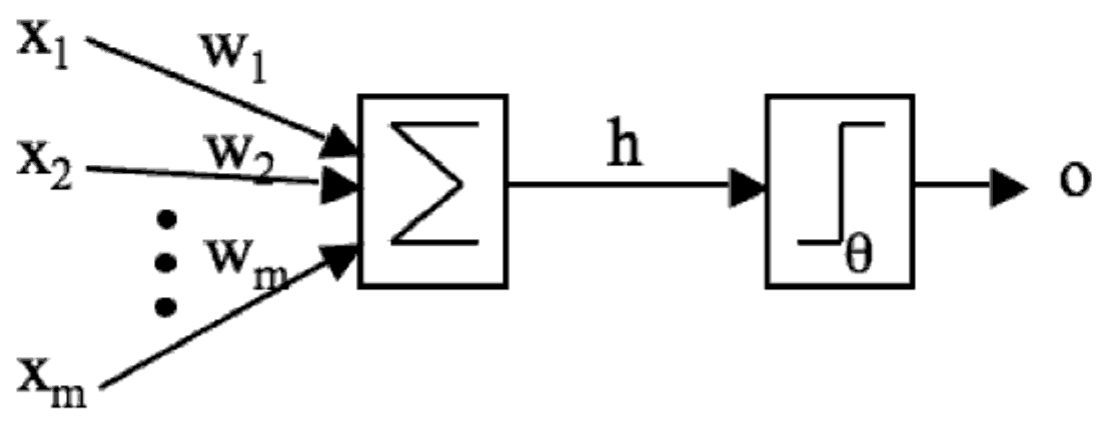
\includegraphics[width=\docwidth]{perceptron}
    \caption[Schema eines Perceptrons / McCulloch-Pitts-Neurons]{Darstellung eines McCulloch-Pitts-Neurons. Die Merkmale $X$ werden mit den Gewichten $W$ multiplziert und in $\sum$ summiert. Wenn $h > \theta$ "`feuert"' das Neuron ($o = 1$) \cite{marsland_opac-b1129336}. \label{fig:perceptron}}
  \end{center}
\end{figure}

Dieser Aufbau kann schon einfache Aufgaben, wie bspw. ein logisches "`UND"', lösen. Jedoch lässt sich schon ein logisches "`XOR"' nicht mehr abbilden. Dafür müssen weitere Schichten von Neuronen (Hidden Layers) hintereinander geschaltet werden - das sog. Multi Layer Perceptron (MPL, Abb. \ref{fig:mlp}).

\begin{figure}[h] 
  \begin{center}
    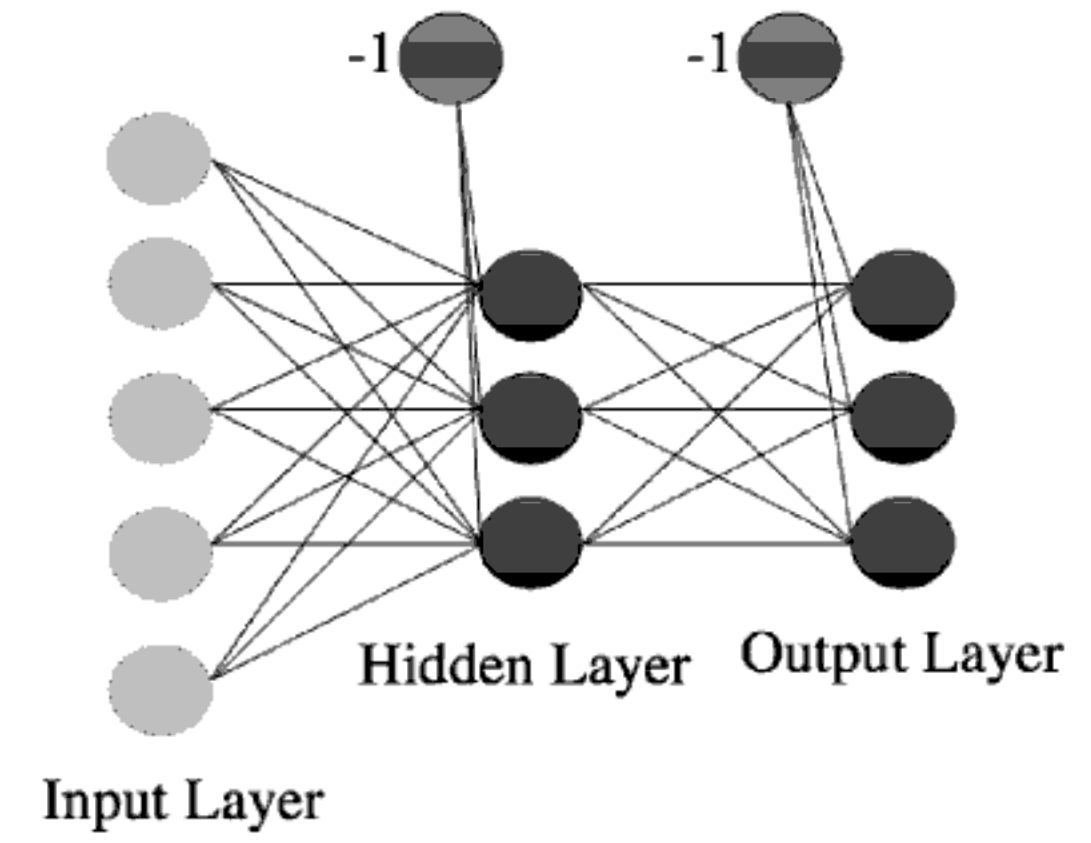
\includegraphics[width=\docwidth]{mlp}
    \caption[Schema eines Multi-Layer-Perceptrons]{Darstellung eines Neuronalen Netzes mit mehreren Schichten (Multi Layer Perceptron, MLP)\cite{marsland_opac-b1129336}. \label{fig:mlp}}
  \end{center}
\end{figure}

Es exisitiert kein bekannter Algorithmus für eine allgemeine Wahl der optimalen initialen Parameter eines KNNs (Gewichte, Anzahl der Hidden Layers). Diese werden initial entweder zufällig gesetzt oder durch Ausprobieren gefunden. Vuckovic et al. \cite{Vuckovic2002349} hatten sich mit diesem Thema genauer beschäftigt.
}

\newcommand{\wavelet}{
Alternativ wäre auch ein Wavelet-Transformation \cite{Chui:1992:IW:163196} möglich gewesen. Beide Ansätze fanden sich in der Literatur Recherche, aus Zeitgründen wurde auf einen Vergleich der Ansätze verzichtet.}